\section{Resultados Finales}

\subsection{Introducción}

Realizamos diferentes gráficos generados pseudo-aleatoriamente con el fin de poder obtener una idea generalizada entre los algoritmos, ya que en las secciones anteriores pudimos
detallar los peores y mejores casos de cada uno. Estos algoritmos fueron generados con una función que recibe como parámetro la cantidad de nodos, y una probabilidad. Dicha función, por cada par de nodos, genera un valor random entre 0 y 100, si este valor está por debajo de la probabilidad recibida como parámetro, unirá dichos nodos, de otra manera, no.\\
Los análisis a realizar serán del estilo cantidad de nodos del conjunto dominante otorgado por cada heurística, comparándolo con el Exacto, y tiempos.\\
Para el GRASP, elegimos correr con k=n/10, ya que después de varias pruebas, nos pareció que con esa cantidad de iteraciones en proporción a la cantidad de nodos encuentra un valor óptimo antes de que el algoritmo entre en lo que denominamos $"$esperando mejor solución que puede no llegar$"$ (remitirse al análisis del GRASP en la sección anterior).\\
Cabe destacar que el algoritmo exacto, se deja de correr para los n $<$ 30 debido a su complejidad. Por esto y porque a partir de ese numero pega saltos tan grandes (en cuanto a tiempos de ejecucion y ciclos de procesador) que se vuelve imposible graficarlo.\\
Para el LocalSearch usamos la estrategia DosPorUno por las razones ya mencionadas en la seccion de ese algoritmo.\\

%En el siguiente grafico se ven las corridas, en nanosegundos, de los 4 algoritmos para un mismo grafo aleatorio con probabilidad 30 (No pusimos grafos con mas de 100 nodos porque al estar corriendo los 4 
%algoritmos para cada grafo el tiempo de corrida se hace demasiado extenso):\\ REVISAR ESTOOOOO CON LO NUEVO ABAJO


\subsection{Por Cantidad De Nodos}

%Generar dos graficos con n$<$200 como eje x y p = 30 (en uno) y p = 50 (en otro)

\begin{center}
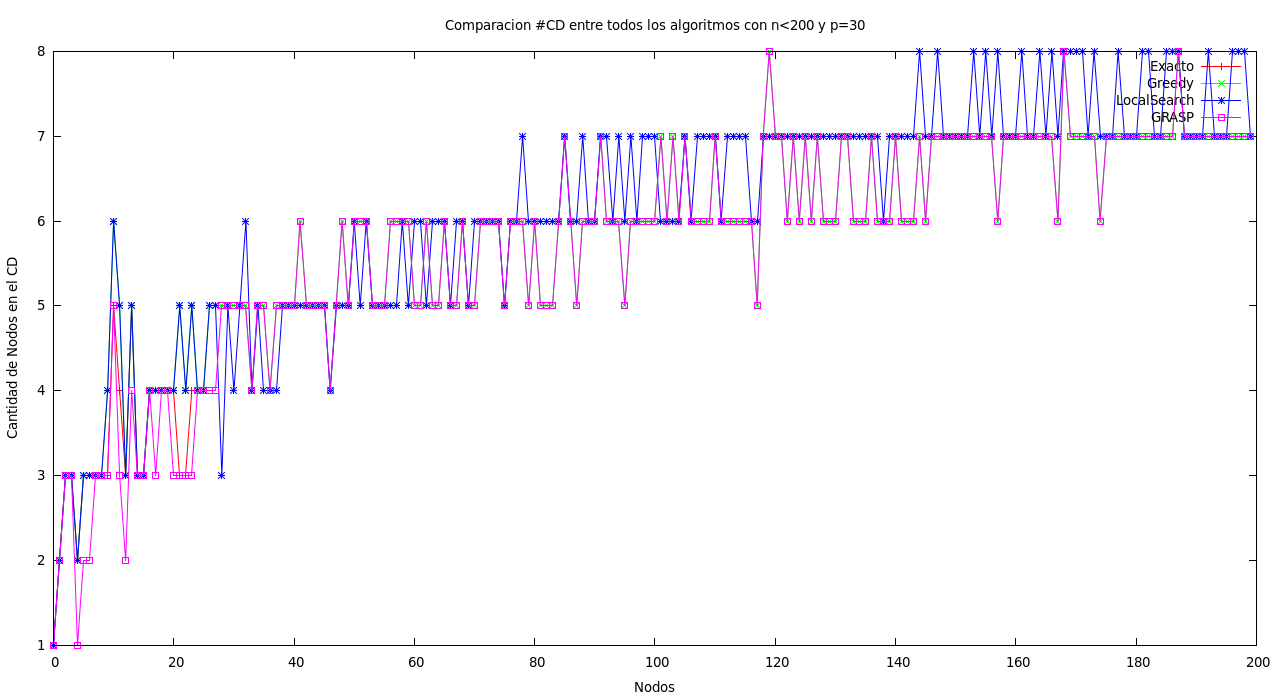
\includegraphics[width=17cm]{./graficos/comparacioncantCDnvariablep30.png}\\
Comparacion por cantidad de nodos con n hasta 200 y p=30
%LISTO
\end{center}


%\begin{center}
%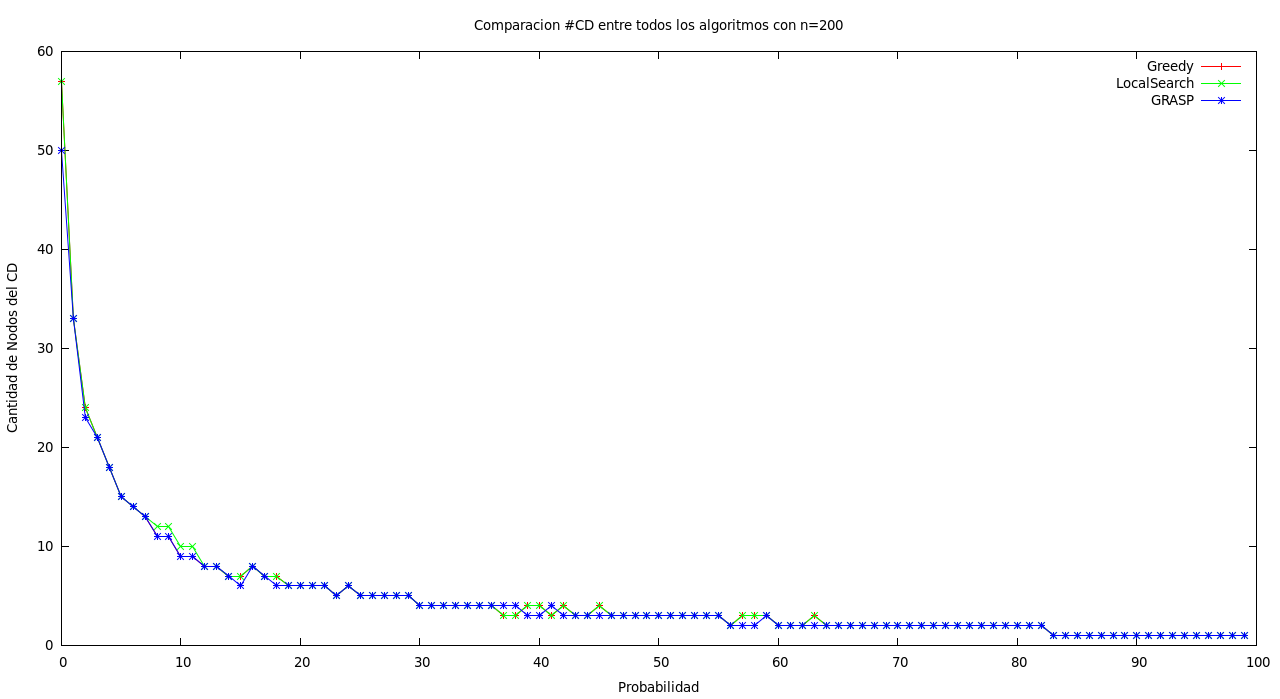
\includegraphics[width=17cm]{./graficos/comparacioncantCDprobvariablen200.png}\\
%Comparacion por cantidad de nodos con n hasta 200 y p=70
%QUEDO HORRIBLE Y NO SALE NINGUN DATO VEMOS SI PONEOMS UNO CON n hasta 100 con p=10
%\end{center}

%Generar dos graficos con p$<$100 como eje x y n = 50 (en uno) y n = 250 (en otro)

\begin{center}
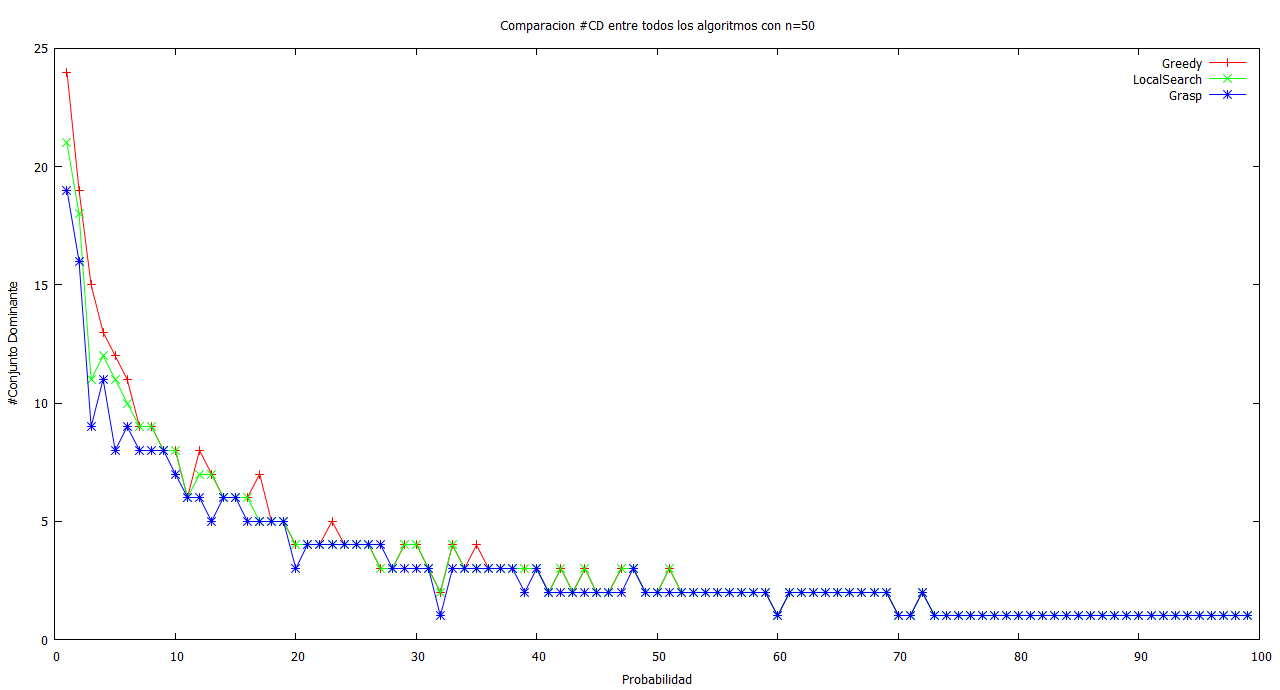
\includegraphics[width=17cm]{./graficos/comparacioncantCDprobvariablen50.png}\\
Comparacion por cantidad de nodos con p hasta 100 y n=50
%LISTO
\end{center}


\begin{center}
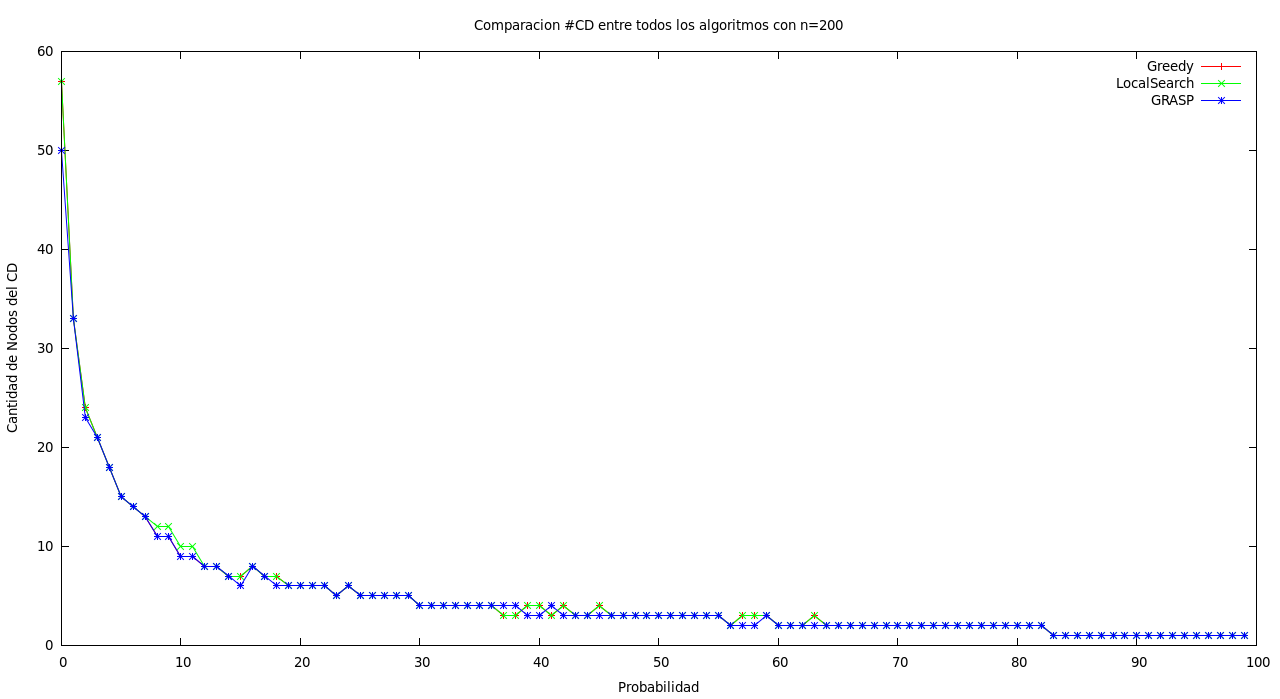
\includegraphics[width=17cm]{./graficos/comparacioncantCDprobvariablen200.png}\\
Comparacion por cantidad de nodos con p hasta 100 y n=200
%LISTO
\end{center}

Como se puede observar en los gráficos, el GRASP se mantiene dominante con la menor cantidad de nodos en su conjunto resultado.
Igualmente, el GREEDY no se aleja demasiado, acompañado por la mejora de Local Search.\\
Otro aspecto a destacar fue que mientras más aristas posee el grafo, el conjunto dominante va a ser más pequeño,
eso es bastante claro ya que habrá más nodos cerca del grado = n-1, por lo que con pocos nodos se encuentra el conjunto dominante.\\
Llevándolo a nuestra primera heurística, es muy probable que el goloso elija bajo su criterio uno de los mejores nodos para el menor
conjunto dominante. Por otra parte, al tener más aristas, la búsqueda local tiene más vecindad para elegir ya que cada nodo se relaciona con
muchos para poder aplicar sus estrategias. Por último, pero no por eso peor, tenemos al GRASP que aplica aleatoriamente los algoritmos previamente
mencionados otorgando una forma distinta (aunque en los gráficos puede verse mejor) de encarar un problema de Conjunto Dominante.


\subsection{Por Tiempo}

%Generar dos graficos con n$<$200 como eje x y p = 30 (en uno) y p = 50 (en otro)

\begin{center}
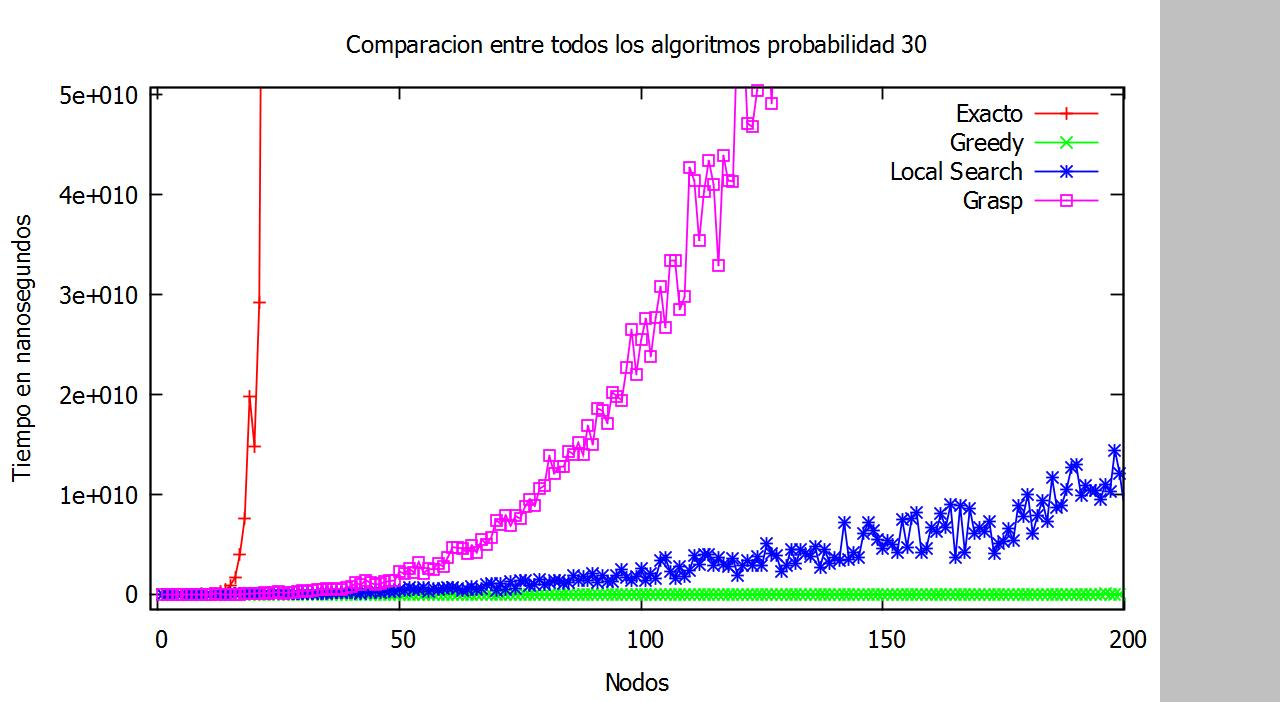
\includegraphics[width=17cm]{./graficos/comparaciontiemponvariablep30.png}\\
Comparacion por tiempo con n hasta 200 y p=30
%LISTO
\end{center}


%\begin{center}
%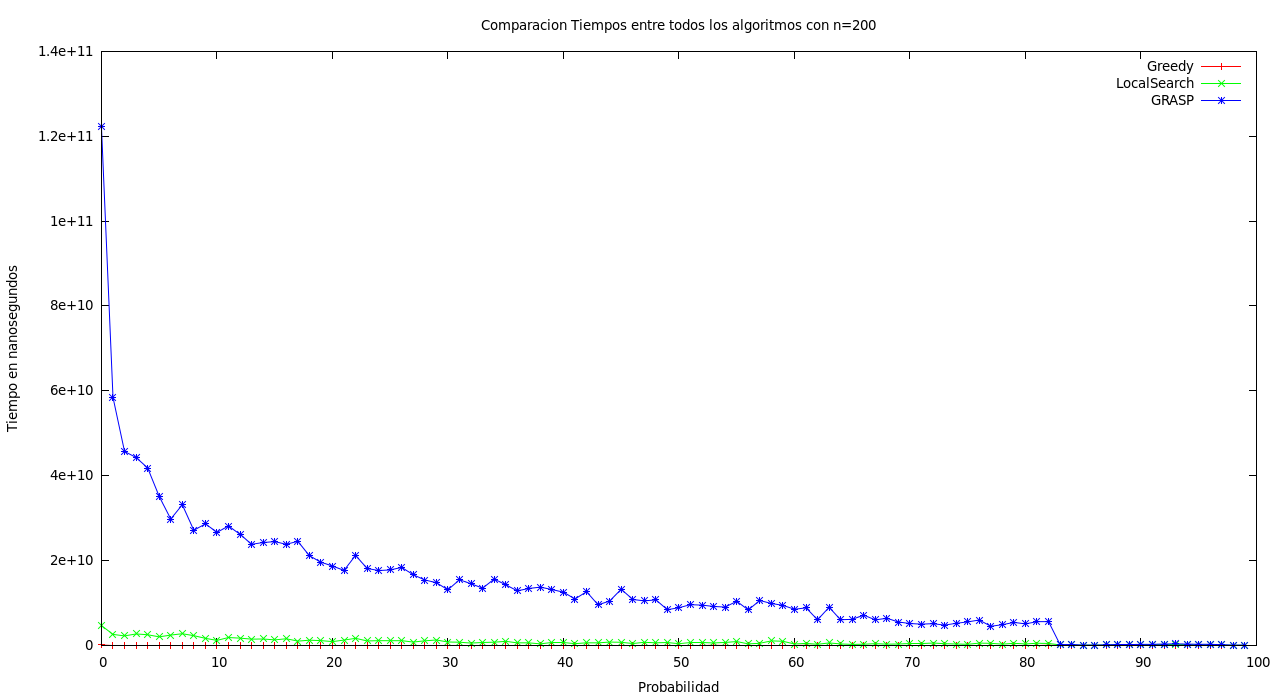
\includegraphics[width=17cm]{./graficos/comparaciontiemposprobvariablen200.png}\\
%Comparacion por tiempo con n hasta 200 y p=70
%QUEDO HORRIBLE Y NO SALE NINGUN DATO VEMOS SI PONEOMS UNO CON n hasta 100 con p=10
%\end{center}

%Generar dos graficos con p$<$100 como eje x y n = 100 (en uno) y n = 250 (en otro)

\begin{center}
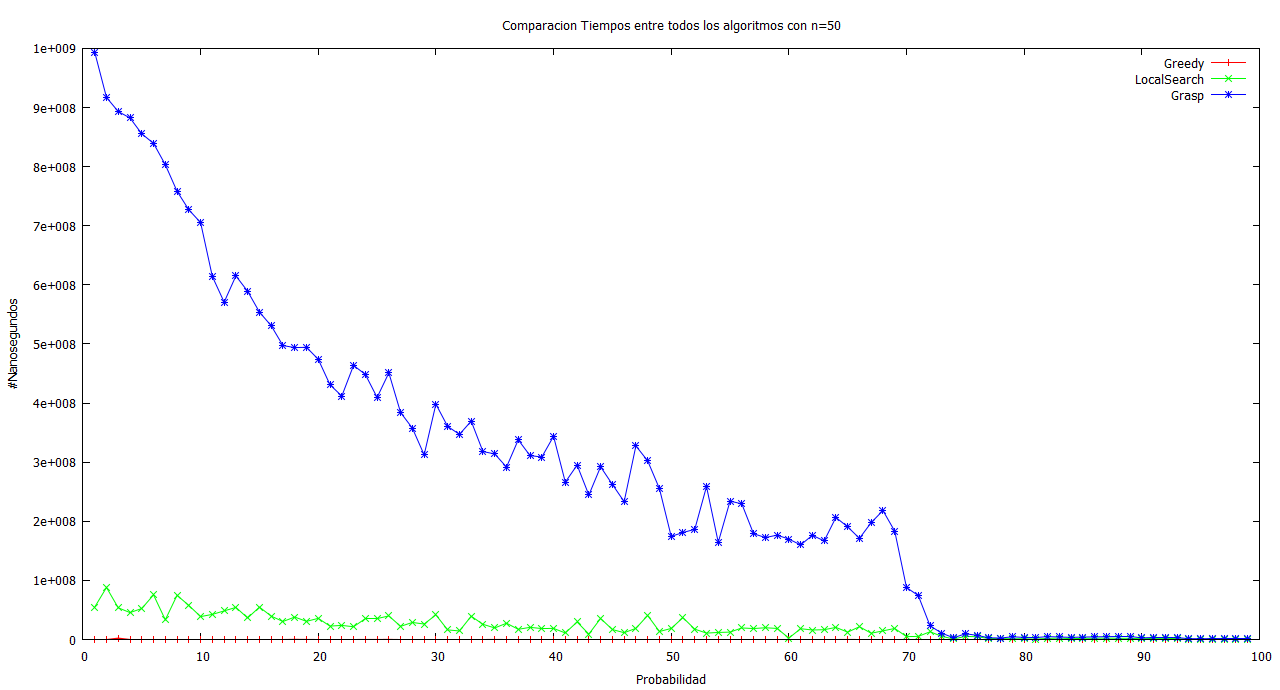
\includegraphics[width=17cm]{./graficos/comparaciontiemposprobvariablen50.png}\\
Comparacion por tiempo con p hasta 100 y n=50
%LISTO
\end{center}


\begin{center}
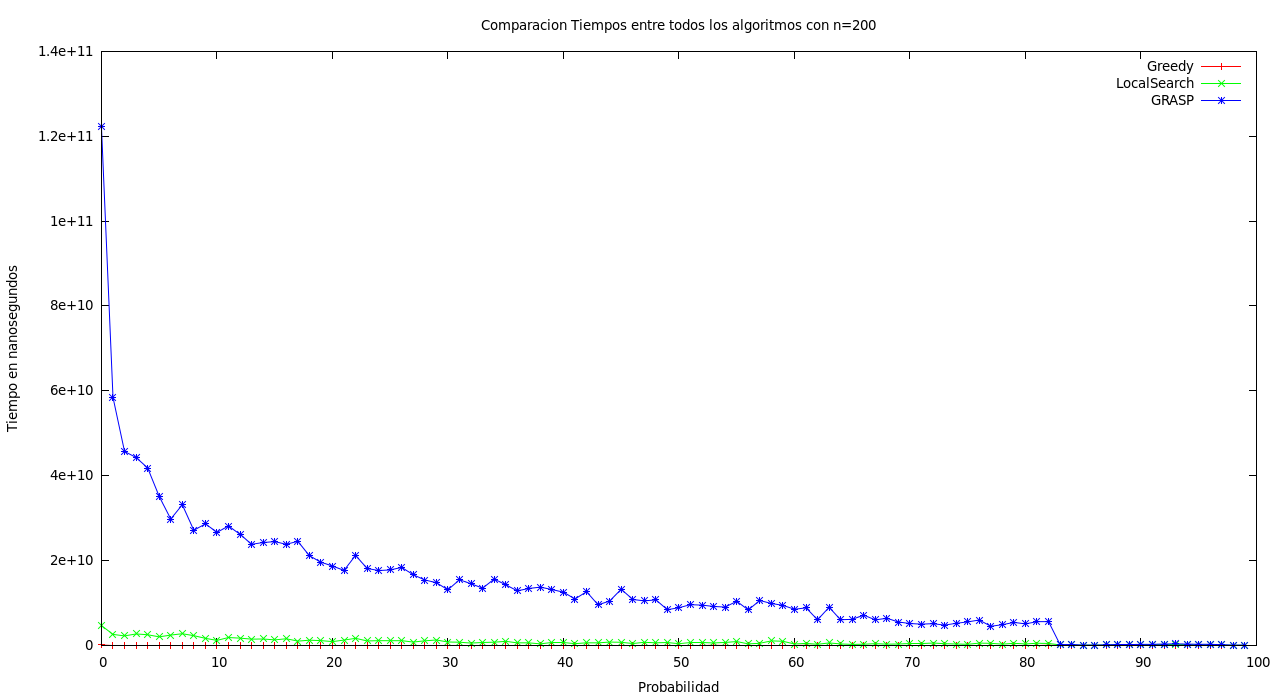
\includegraphics[width=17cm]{./graficos/comparaciontiemposprobvariablen200.png}\\
Comparacion por tiempo con p hasta 100 y n=200
%LISTO
\end{center}

En cuanto a la relación cantidad de nodos, vemos como GRASP tarda mucho más que el resto de los algoritmos 
y esto es debido a la complejidad, la que queda bien evidenciada en el primer gráfico. A mayor costo, mejores resultados.\\
De los gráficos recién mencionados, podemos extraer que a mayor densidad, el algoritmo tarda menos.
Esto tiene sentido porque es más probable que la cardinalidad del conjunto dominante sea uno, o que sea muy chico.
De esta forma, el Greedy seleccionará el de mayor grado, que será muy cercano a n-1 y además habrá varios con este grado, y en pocas iteraciones
encontrará un conjunto dominante, lo que queda poco trabajo para el LocalSearch por tener una vecindad chica.
Por parte del GRASP, pasará lo mismo.\\
Finalmente cabe mencionar que el algoritmo GRASP tarda siempre más que el de búsqueda local y este ultimo más que el
greedy. Esto se debe a que el de búsqueda local ejecuta el greedy y luego intenta mejorar la solución, y el GRASP realiza una
determinada cantidad de iteraciones en las que ejecuta, en cada una, el greedy y lo mejora con búsqueda local.

\subsection{Cotas}

\begin{center}
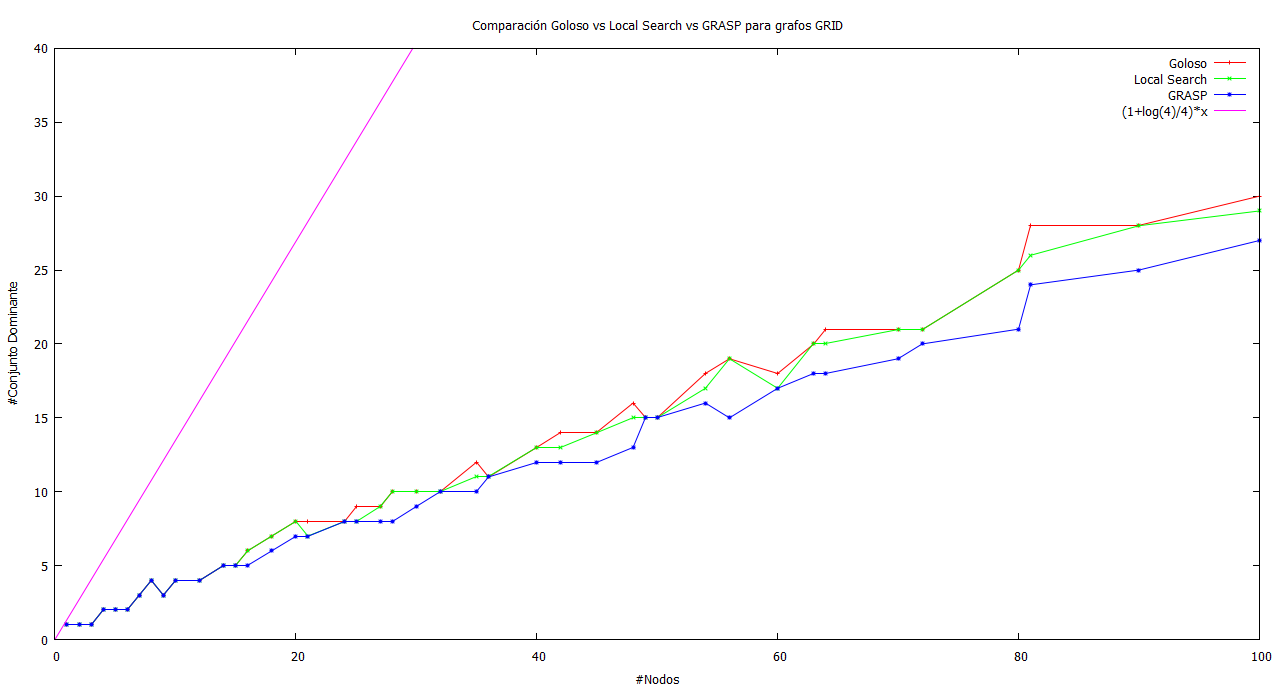
\includegraphics[width=17cm]{./graficos/comparacion_heuristicas_cd.png}\\
Comparacion por cantidad de nodos con cota de grafos conexos$^{[3]}$
%LISTO
\end{center}

La cota del tamaño del conjunto dominante para los grafos conexos$^{[3]}$ es:
Tamaño del conjunto dominante \leq (\frac {1+ln(1+\delta)}{1+\delta})n 

Como se puede ver en el gráfico, no solo el GRASP encuentra un mejor resultado con respecto a los otro algoritmos, si no que también
podemos asegurar que el resto de las heurísticas se alejan de igual manera de la cota mencionada.


\section{Conclusiones}
Para finalizar, quremos concluir que si bien las heurísticas no poseen siempre el resultado óptimo
suelen acercarse bastante, y si sabemos información sobre nuestro grafo podemos anticipar resultados 
o titempos. Esto es necesario ya que el exactó probó no ser factible para n no muy grandes.\\
Finalmente, para uso práctico podemos recomendar utilizar el algoritmo de búsqueda local por sobre el greedy para obtener
una solución razonablemente buena en poco tiempo, ya que la puede mejorar con un costo adicional bastante bajo. Para problemas
en los que se necesite mayor precisión, se puede aplicar GRASP variando el parámetro k y
teniendo en cuenta lo mencionado anteriormente.



%------------------------------------------------------------------VERSION ANTERIOR---------------------------------------------------------------------------------
\begin{comment}
\subsection{Exacto - Goloso}

Como vimos anteriormente el algoritmo Exacto tiene complejidad exponencial mientras que el Goloso polinomial. Es decir que para valores de entrada grandes el Goloso va a costar mucho menos ciclos. Por otra parte el Greedy puede devolver conjuntos dominantes no mínimos (es decir un conjunto dominante tal que exista un conjunto con menor cantidad de nodos que también sea dominante) mientras que el Exacto absolutamente siempre va a devolver el mínimo. \\
Teniendo en cuenta estos conceptos, para saber que algoritmo nos conviene usar tendríamos que tener en cuenta varias cosas. Si sabemos que las instancias de entrada rara vez serán con mas de un nodo del mismo grado, no nos afecta significativamente que el algoritmo nos devuelva esporádicamente resultados subóptimos y necesitamos que el algoritmo sea veloz, claramente la mejor opción es el Greedy. Ya que dificilmente fallaría (porque casi siempre vendrían grafos con todos nodos de distintos grados), funciona mucho más rápido que el exacto y el caso en que falle no sería decisivo. \\
Ejemplo:\\
Un ejemplo de la vida real de este caso podría ser si quisiese elegir a los referentes políticos de cada provincia de forma tal que representen a toda la población a través de la influencia en esta que ejercen . Donde influencia se entiende como gente que lo apoya y cada persona puede apoyar a mas de uno (esto se obtuvo a través de encuestas). El problema lo abstraeríamos a grafos diciendo que cada nodo es una persona y estas se relacionan si una apoya la otra (no importa quien a quien ya que entendemos que si un ciudadano apoya a un candidato político es porque este también apoyaría al ciudadano, un poco utópicos lo se). En este caso como por lo general los dirigentes políticos zonales tienen influencia gracias a los partidos políticos a los que pertencen y estos suelen diferir entre sí en la cantidad de adherentes (es muy raro que dos partidos tengan exactamente la misma cantidad de adherentes) entonces en la gran mayoría de los casos los grafos van a estar compuestos todos por nodos con distinto grado y además van a ser datos de entrada muy grandes (ya que cada provincia contiene como mínimo 100 mil habitantes) por lo tanto en este caso sería muchísimo mejor utilizar el Greedy. \\
En cambio si no me importa mucho el tiempo de proceso, se que los datos de entrada no van a ser muy grandes y necesito que el resultado sea siempre el mejor me conviene usar el exacto. Un caso de esto podría ser si mediante un mapa del circuito eléctrico de una ciudad del interior (es decir una ciudad chica) quiero obtener los puntos desde los cuales puedo llegar a todo el resto del tramado eléctrico para mejorar los transistores, para esto mediante la obtención del conjunto dominante mínimo obtendríamos estos puntos y los devolveríamos. Si consideramos que mejorar cada transistor nos cuesta cientos de miles de pesos es primordial que el resultado sea exacto y como solo deseamos correrlo una vez no es tan importante el tiempo que pueda tardar. Por eso en este caso la mejor opción sería el algoritmo exacto. \\

En el siguiente gráfico podemos apreciar la diferencia en ciclos entre estos algoritmos para distinta cantidad de nodos. Se puede ver claramente que a medida que el grafo tiene mas nodos la diferencia crece abisamalmente. Para el caso del exacto no pusimos los valores para todas las cantidades debido a que se hacía poco visible como evolucionaba la linea del goloso ya que el exacto alcanzaba valores muy muy grandes. 
\begin{center}
  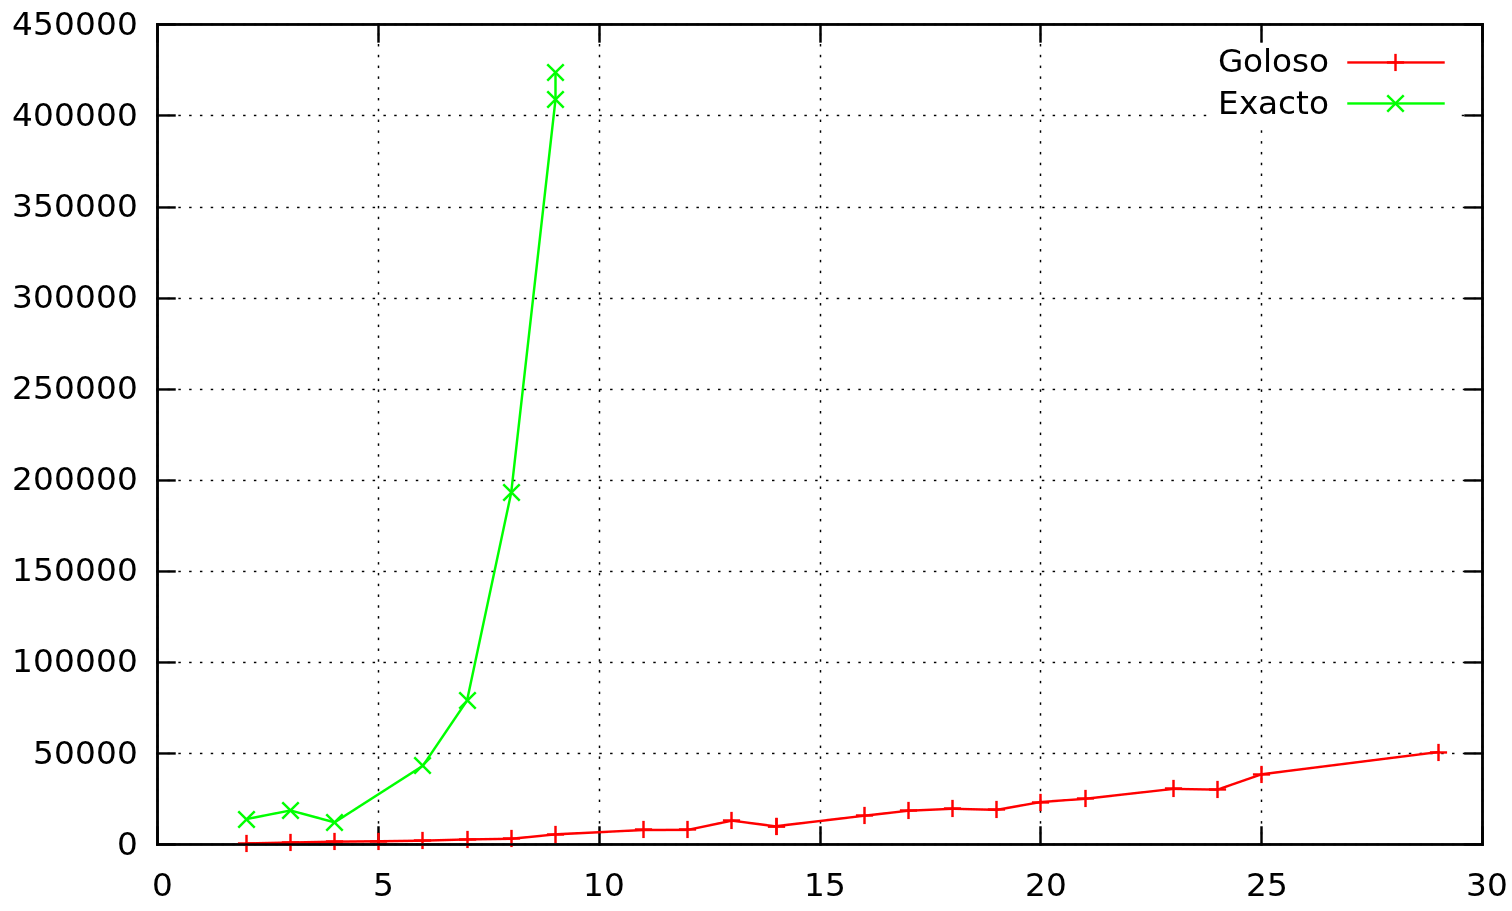
\includegraphics[width=12cm]{./graficos/comp_exacto_goloso.png}
\end{center}


\subsection{Exacto - Goloso - Local Search}
En ésta sección vamos a comparar tanto las soluciones obtenidas como el consumo de tiempo en éstos tres algoritmos. Decidimos hacerlo de ésta forma, y no separadamente, ya que el algoritmo greedy es parte (al menos, en nuestro caso), de la búsqueda local, y utilizamos el exacto para saber si las soluciones obtenidas son buenas o no. Por lo tanto, analizaremos los tres casos juntos. Para ello, vamos a ayudarnos de dos gráficos, donde podemos ver la cardinalidad de las soluciones para distinta cantidad de nodos, y el tiempo tomado para resolverlos. \\
\begin{center}
  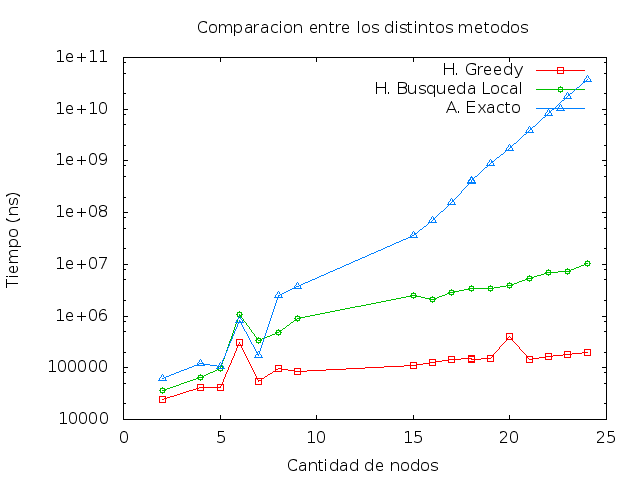
\includegraphics[width=12cm]{./graficos/local_comparacion.png}
\end{center}
Como vimos en el análisis anterior, para instancias muy pequeñas, y donde la exactitud es preponderante, el algoritmo exacto es el más adecuado a utilizar, ya que la diferencia de tiempo es muy poca, pero la diferencia de la solución podría ser considerable. En cambio, para entradas un poco más grandes (como podemos apreciar en el gráfico, de una diferencia de 5 nodos), ya no es conveniente utilizar el algoritmo exacto, ya que el tiempo que consume es exponencial a su cantidad de nodos, como podemos ver en el gráfico 1. En cambio, es recomendable utilizar alguno de los otros dos algoritmos que estamos analizando. \\
La gran diferencia entre el tiempo utilizado para encontra una solución con la búsqueda local y el algoritmo greedy, a pesar de tener complejidades parecidas, la podemos adjudicar a que en la búsqueda local, el proceso de encontrar soluciones "locales" se repite varias veces, y para varios métodos que tienen la misma complejidad (como ya dijimos antes, $n^2$), así que si bien consume más tiempo que la heurística golosa, ésta crece de forma polinomial, y es, por lejos, mucho mejor que la solución exacta, y muchas veces, como podremos analizar en párrafo y gráfico siguiente, nos ofrece una solución igual a la exacta o cuya cardinalidad difiere en 1 o 2 nodos únicamente. \\
Cuál de ellos es una pregunta que debe ser respondida según la situación y la exactitud de la solución que se busque, a partir del análisis de los gráficos 1 y 2 de ésta sección, donde se analiza la cantidad de soluciones y el tiempo demandado para encontrarlas. 

\begin{center}
  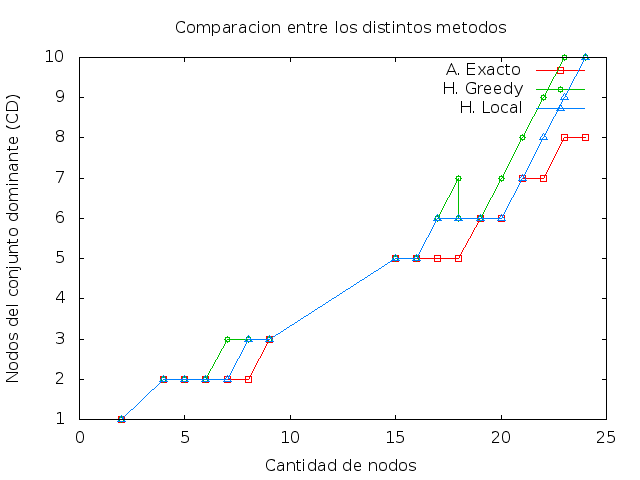
\includegraphics[width=12cm]{./graficos/local_comparacion_soluciones.png}
\end{center}

Por un lado, si sólo se desea encontrar un conjunto dominante, podemos utilizar la solución golosa, que es la más rápida de las 3 ya que no depende de ninguna otra solución. Por su parte, si la instancia es muy grande, pero deseamos que la solución sea lo más óptima posible, y que el tiempo de resolución sea polinomial, debemos utilizar la búsqueda local, ya que ha demostrado ser al menos tan mala como la solución greedy, aún en casos cuando la solución que le pasamos es el grafo entero (es decir, tomamos como conjunto dominante a todo el grafo, por más malo que eso sea). 


\subsection{Exacto - Goloso - Local Search - GRASP}

A continuación haremos una comparación masiva de los 3 primeros algoritmos contra GRASP.
Corremos distintos grafos con GRASP k=15, y los mismos grafos con los otros algoritmos.
\begin{center}
  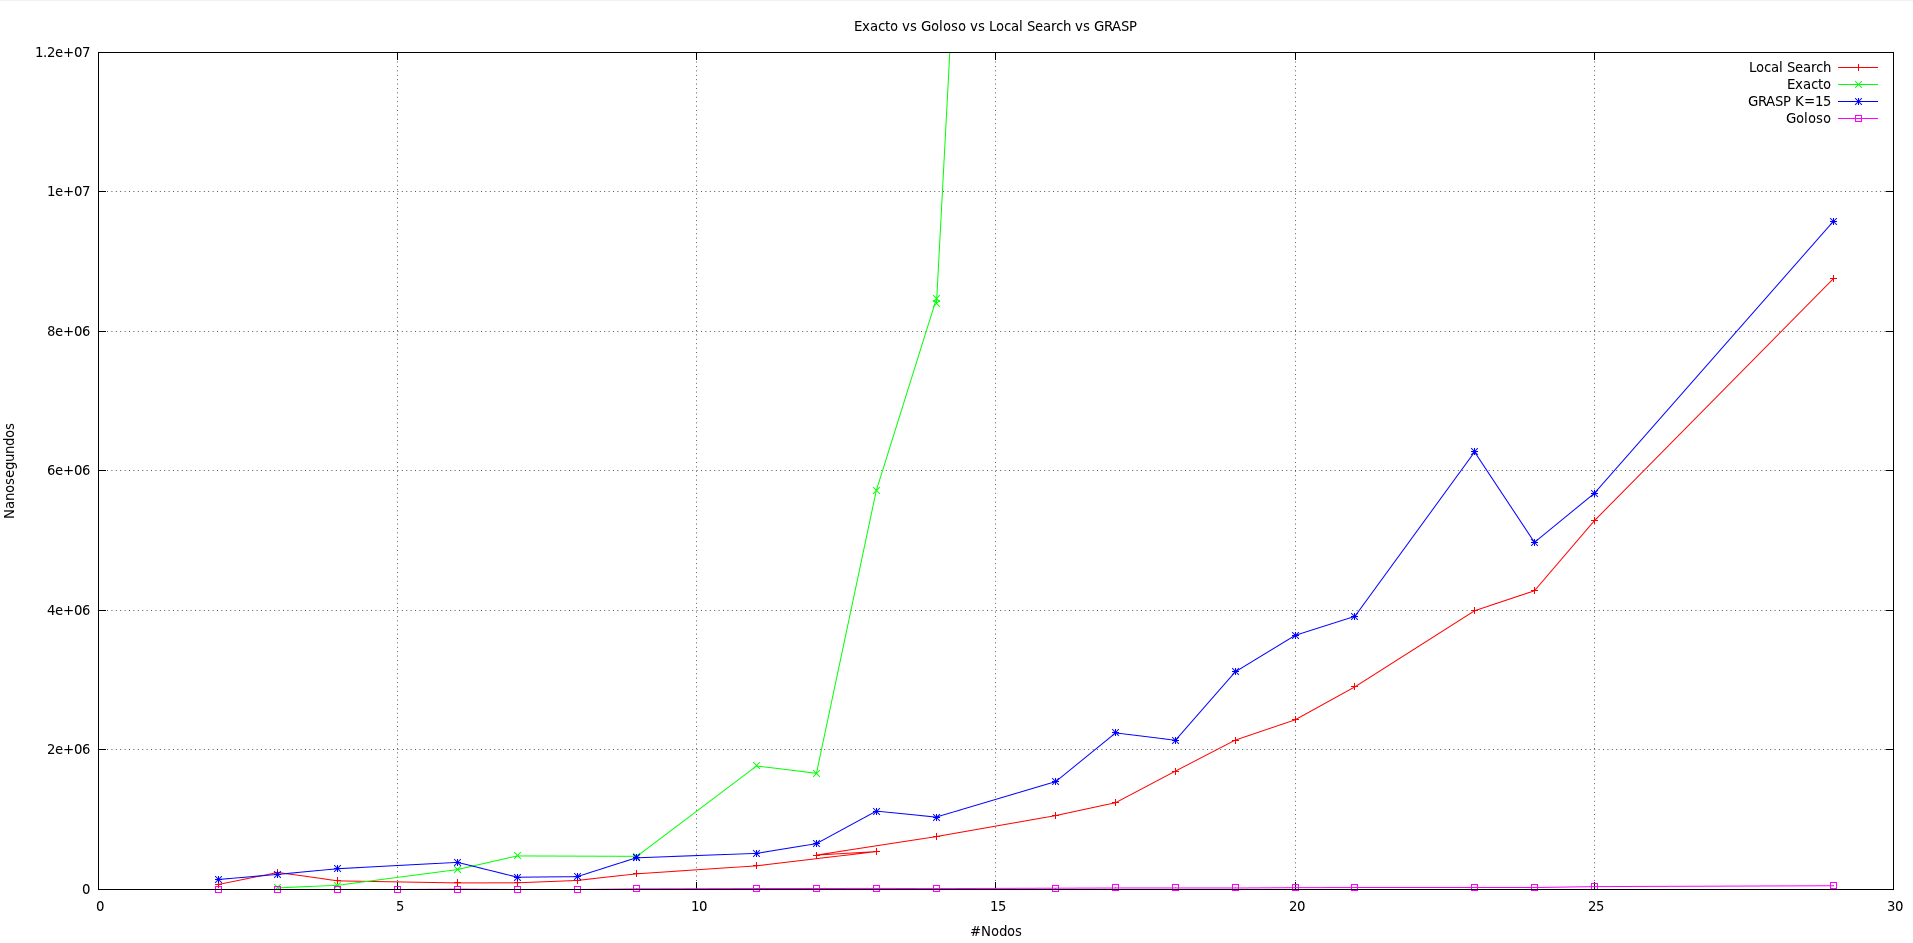
\includegraphics[width=15cm]{./graficos/todosVStodos.png}
\end{center}
Como vimos antes no hay una gran variación de tiempo de procesamiento más allá la diferencia entre la exponencialidad del Exacto contra la polinomialidad del resto, por lo tanto queremos aclarar que en caso de tener que resolver este
problema a través de una Heurística, fuertemente recomendamos ejecutar GRASP, ya que no existe gran diferencia de tiempos, y el algoritmo en el peor de los casos devuelve la misma cantidad de nodos que el goloso. Sin embargo, como ya 
mencionamos antes la cantidad de soluciones que puede devolver el GRASP se ve multiplicada por k, y a cada una de estas k soluciones se lo intenta mejorar localmente. Es por eso que, si sabés datos de la entrada 
del grafo en donde greedy pueda llegar a devolver un resultado lejos del exacto, es recomendable utilizar GRASP ya que aumentás las posibilidades y probabilísticamente podés conseguir una mejor solución.
\end{comment}
